\documentclass[12pt]{article}

\usepackage[english]{babel}
\usepackage[utf8x]{inputenc}
\usepackage{pdfpages}
\usepackage{lastpage} % Required to determine the last page for the footer
\usepackage{extramarks} % Required for headers and footers
\usepackage{graphicx} % Required to insert images
\usepackage{listings} % Required for insertion of code
\usepackage{courier} % Required for the courier font

% Margins
\topmargin=-0.45in
\evensidemargin=0in
\oddsidemargin=0in
\textwidth=6.5in
\textheight=9.0in
\headsep=0.25in

\linespread{1.1} % Line spacing

\newcommand{\Title}{Design Documentation} % Assignment title
\newcommand{\Class}{Cos\ 301} % Course/class

\begin{document}

	\vspace{4em}
	
	\begin{center}%
	
	  \LARGE \bf \Title \\[4em]
	  \LARGE {\bf Group 1}\\[1em]
	  \LARGE {\bf Group Members:}\\[2em]
	  \large
	  
	     Mbulungo Musetsho				(10176382) \\[1em]
	     Ndivhuwo Ntambeleni			(10001183) \\[1em]
	     Pule Legodi                                (29302732) \\[1em]
	    	%Enter your details below just as the one above
	    
	\end{center}%
	

	\newpage
	\tableofcontents
	
	\newpage
	\section{Background}
	
		\vspace{0.2in}
	
				 %We must give an introduction of this document
		
		 
	
	\section{Vision}
	
		\vspace{0.2in}
		
			 		 %We must briefly describe the purpose of this document
				
	
	\section{Software Architecture Design}
			%This section needs to demonstrate how the system will be able, within designed software architecture, to address the non-functional requirements.
		\vspace{0.2in}
		
		\subsection{Choices of Technologies}
		%Please refer to the guideline document for some of the items that must be included in this part.
			\vspace{0.2in}
		
		
		\subsection{Chosen Frameworks}
				%Please refer to the guideline document for some of the items that must be included in this part.
					\vspace{0.2in}	
			
		
		\subsection{Chosen Protocols}
				%Please refer to the guideline document for some of the items that must be included in this part.
			\begin{enumerate}
	                    \item Simple Object Access Protocol (SOAP) \\*
	                    All systems (devices) should be able to access the system’s content through the SOAP-based web services. 
	                        \begin{enumerate}
	                            \item The devices (systems) will send a request, procedure call, or a message such as getMark to search or retrieve information (average mark for the module, number of distinctions) through the SOAP-based web services.
	                            \item The SOAP-based web service will process the request or message and send a response to the devices (systems) in a form of a structured XML-based data.
	                        \end{enumerate}
	                    \item Lightweight Directory Access Protocol (LDAP)
	                        \begin{enumerate}
	                            \item It is used to authenticate the system users (Lecturers, Students, and Teaching Assistants) on login for single Sign On.
	                            \item It is used to retrieve the student’s personal details and class lists, including courses assigned to lectures and students.
	                            \item It is used to retrieve system users roles such as, is the user a Lecturer, Student, or teaching assistant for the Module
	                        \end{enumerate}
	                    \item  Hypertext Transfer Protocol over Secure Socket Layer (HTTPS and HTTP)
	                        \begin{enumerate}
	                            \item Used to send and retrieve sensitive data(marks and modules) through a secured (HTTPS) channel.
	                            \item Used to send a GET and POST requests to the web server and web services. Such as adding or updating a student mark.
	                        \end{enumerate}
	                        
              		\end{enumerate}
			\vspace{0.2in}
			
		
		\subsection{Chosen Libraries}
				%Please refer to the guideline document for some of the items that must be included in this part.
			\vspace{0.2in}

			
	\section{Application Design}
				%must address functional requirements as specied in re-quirements specification.
			\vspace{0.2in}
					
		\subsection{Lower Levels of Granularity Specification}
				
		\vspace{0.2in}
		
		\subsection{API Specifications}
						%UML interfaces and class diagrams for inputs and outputs, etc
				\vspace{0.2in}
				
		\subsection{System Class Diagrams }%Ndivhuwo Nthambeleni
		%Class Diagram for assessment marking and assessment aggregation
				
				\begin{figure}[h]
						\centering
						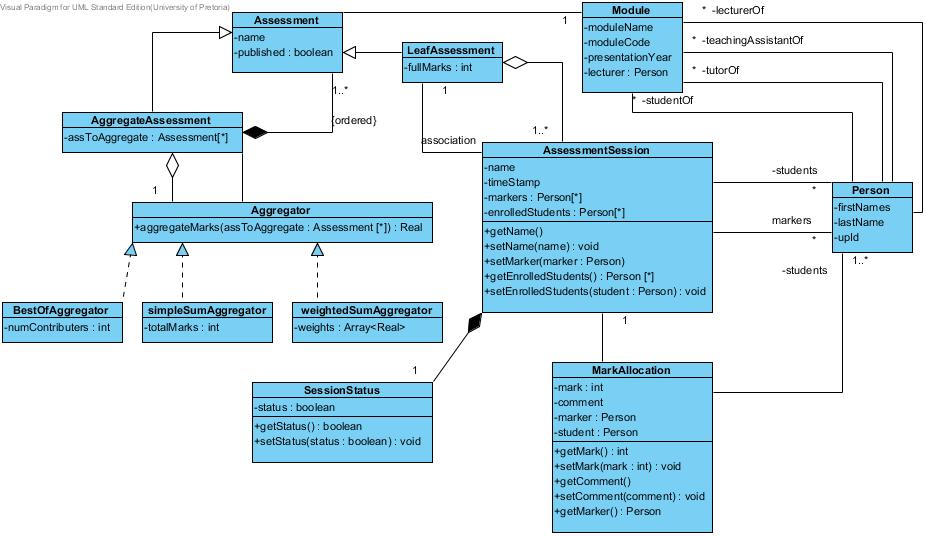
\includegraphics[width=6in, height=4in]{Pictures/MiniPhase2ClassDiag.jpg}
						\caption{Assessment Class Diagram}
				\end{figure}
						%These class diagrams must include attributes, methods and relationships
						
				\vspace{0.2in}
		
		\subsection{System Process Specification}%Mbulungo Muusetsho
						%Sequence and activity diagrams for detailed system process specifications
						\begin{figure}[h]
										\centering
										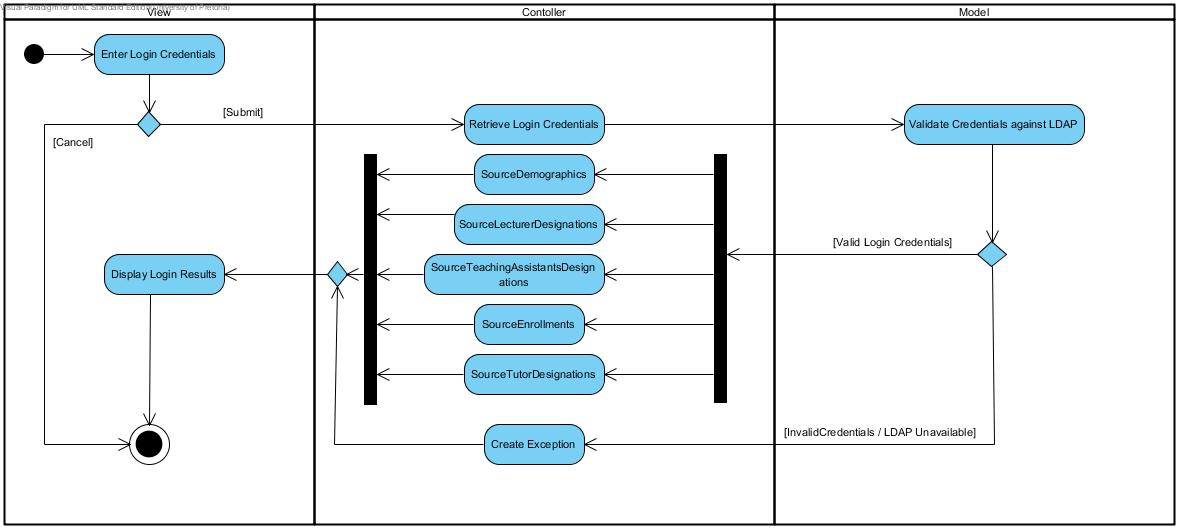
\includegraphics[width=6in, height=4in]{Pictures/LoginActivityDiagram.jpg}
										\caption{User Log In Activity Diagram}
						\end{figure}
						\begin{figure}[h]
										\centering
										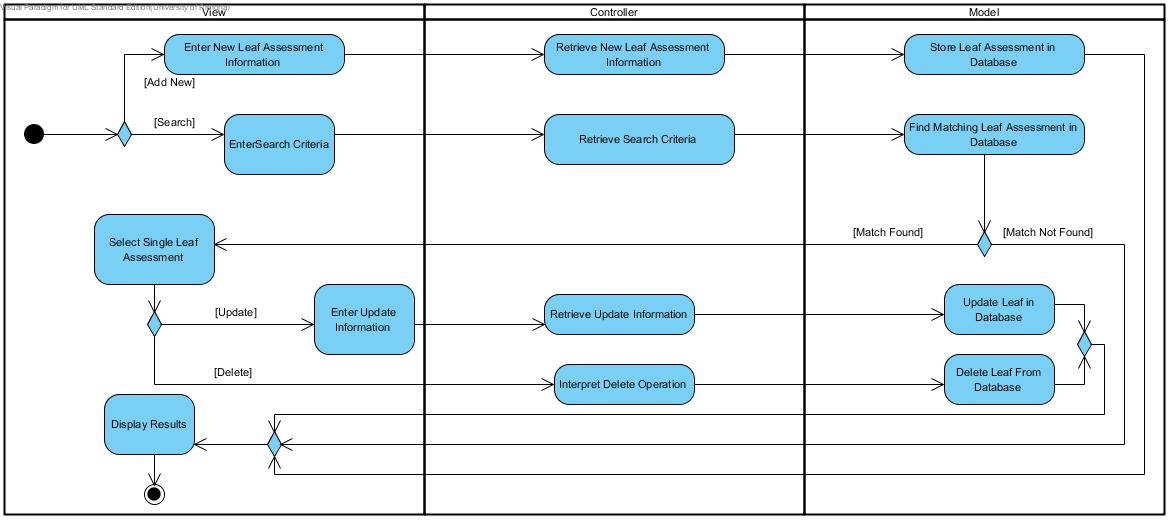
\includegraphics[width=6in, height=4in]{Pictures/LeafAssesmentActivityDiagram.jpg}
										\caption{Leaf Assessment Activity Diagram}
						\end{figure}
						\begin{figure}[h]
										\centering
										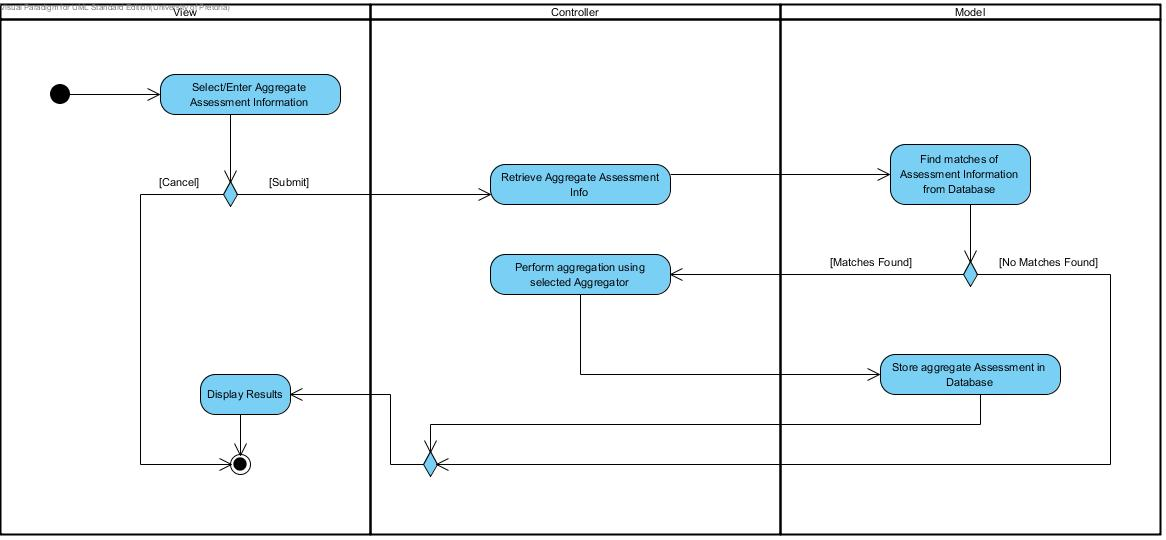
\includegraphics[width=6in, height=4in]{Pictures/AggregateAssesmentActivityDiagram.jpg}
										\caption{Aggregate Assessment Activity Diagram}
						\end{figure}
						\begin{figure}[h]
										\centering
										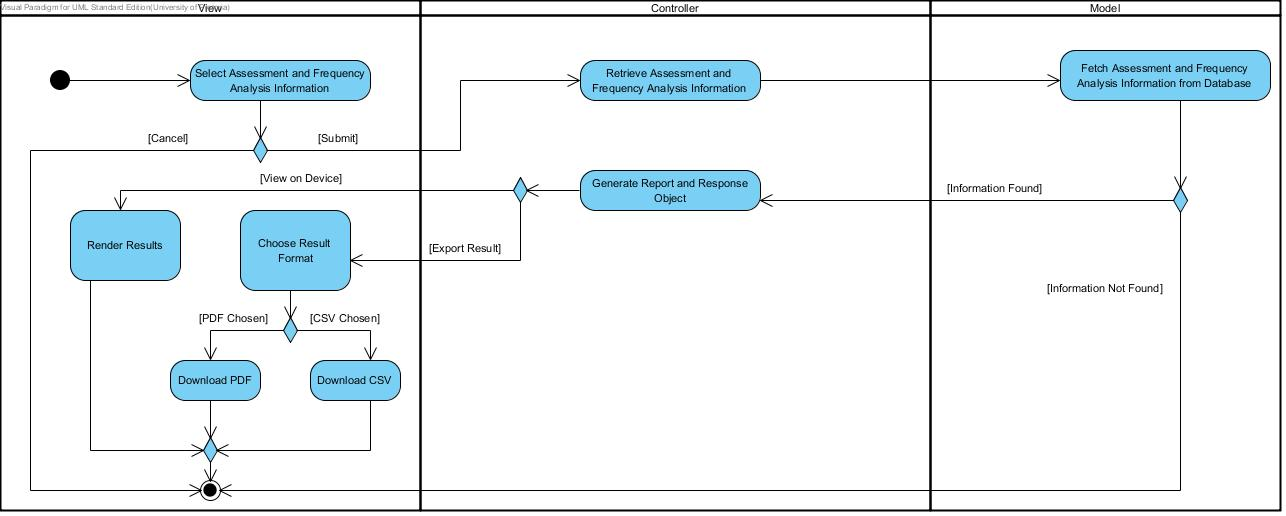
\includegraphics[width=6in, height=4in]{Pictures/AssessmentReportActivityDiagram.jpg}
										\caption{Assessment Report Activity Diagram}
						\end{figure}
						\begin{figure}[h]
										\centering
										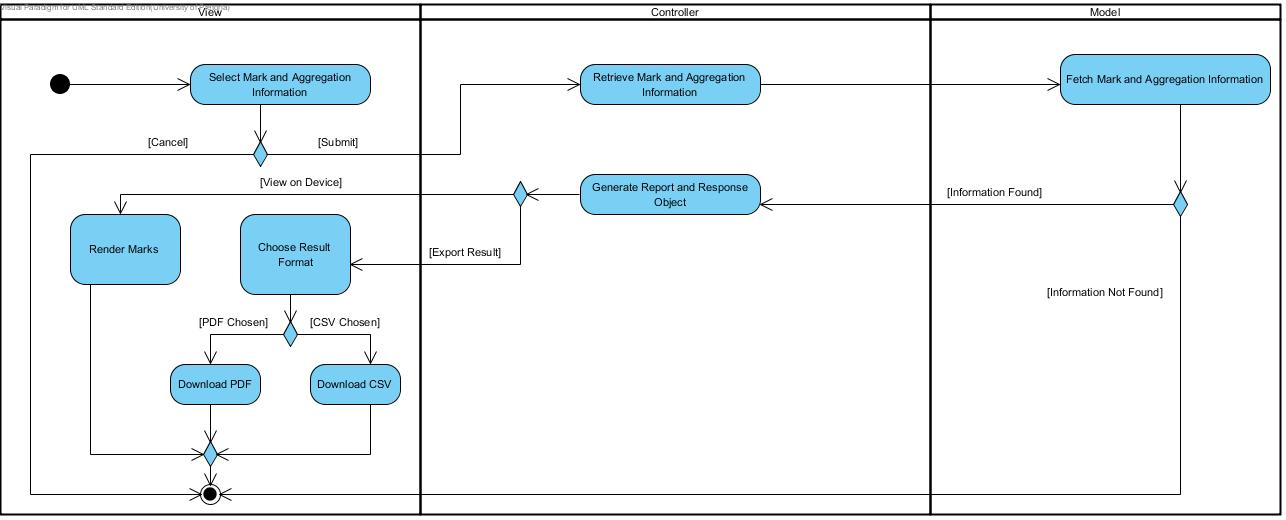
\includegraphics[width=6in, height=4in]{Pictures/StudentMarksReport.jpg}
										\caption{Student Marks Report Activity Diagram}
						\end{figure}
						\begin{figure}[h]
										\centering
										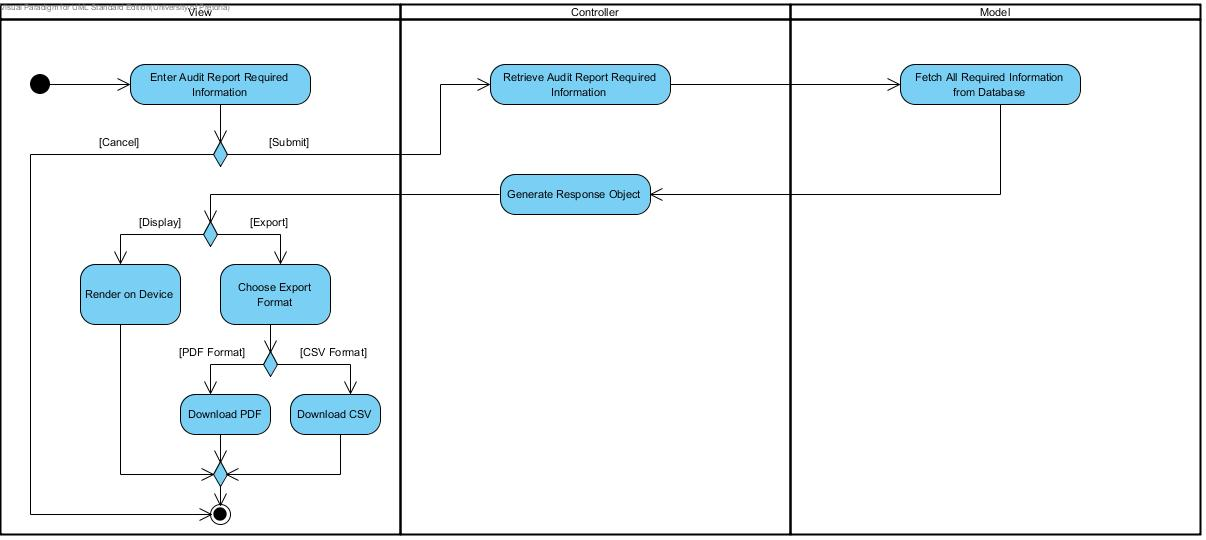
\includegraphics[width=6in, height=4in]{Pictures/AuditReportActivityDiagram.jpg}
										\caption{Audit Report Activity Diagram}
						\end{figure}
				\vspace{0.2in}
		
		\subsection{User Interface Designs} %MatthewHughes and Ndivhuwo Nthambeleni
						%This includes work-flow specifications
				\vspace{0.2in}
		
		\subsection{Database Desgin} %Lutfiya
						%Database tables, etc
						
				\vspace{0.2in}
			
			
	
	\section{Open Issues}
	
		\vspace{0.2in}
		
		
	\newpage
	\section{Glossary}
	
		\vspace{0.2in}
		
			
	
	
\end{document}
